\subsection{Versuchsaufbau}\label{subsec:Versuchsaufbau}
Für den Versuchsaufbau wurde der BLDC mit einer asynchronen Maschine (ASM) gekoppelt, welche über einen Frequenzumrichter angesteuert wird und netzspeisefähig ist. Die ASM simuliert bei den nachfolgenden Versuchen die Last.


\begin{figure}[H]
	\begin{center}
		\includegraphics[height=70mm]{Versuchsaufbau/Schema.png}
		\caption{Schema Versuchsaufbau}
		\label{fig:Schema}
	\end{center}
\end{figure}

Um die verschiedene Versuche auszuwerten, wurde je nach Versuch verschiedene Gössen gemessen.
Die \textbf{Spannung} und der \textbf{Strom} wurde zwischen der Ansteuerung und dem B6-Gleichrichter gemessen. Die \textbf{Drehzahl} wurde mithilfe eines Oszillator ausgewertet. Dabei wurde dieser direkt an einem Hallsensor angehängt, welcher vier Impulse pro Umdrehung generiert. Die \textbf{Leistung} wurde mithilfe eines Power-Analyzers zwischen der ASM und dem Frequenzumrichter gemessen. Der \textbf{Drehmoment-Sollwert} wurde digital mit einem Mikrocontroller erzeugt und auf die Ansteuerung gegeben. Die \textbf{Motor-} und \textbf{Controller-Temperatur} wurden direkt am Computer ausgelesen, welcher an der Ansteuerung angeschlossen ist.\\

Wie auf dem Schema auf der Abbildung \ref{fig:Schema} ersichtlich, erfolgt die Energieversorgung durch das Netz und wird auf einen Variac (Abbildung \ref{fig:Variac}) geführt, welcher nachfolgend abgebildet ist.

\begin{figure}[H]
	\begin{center}
		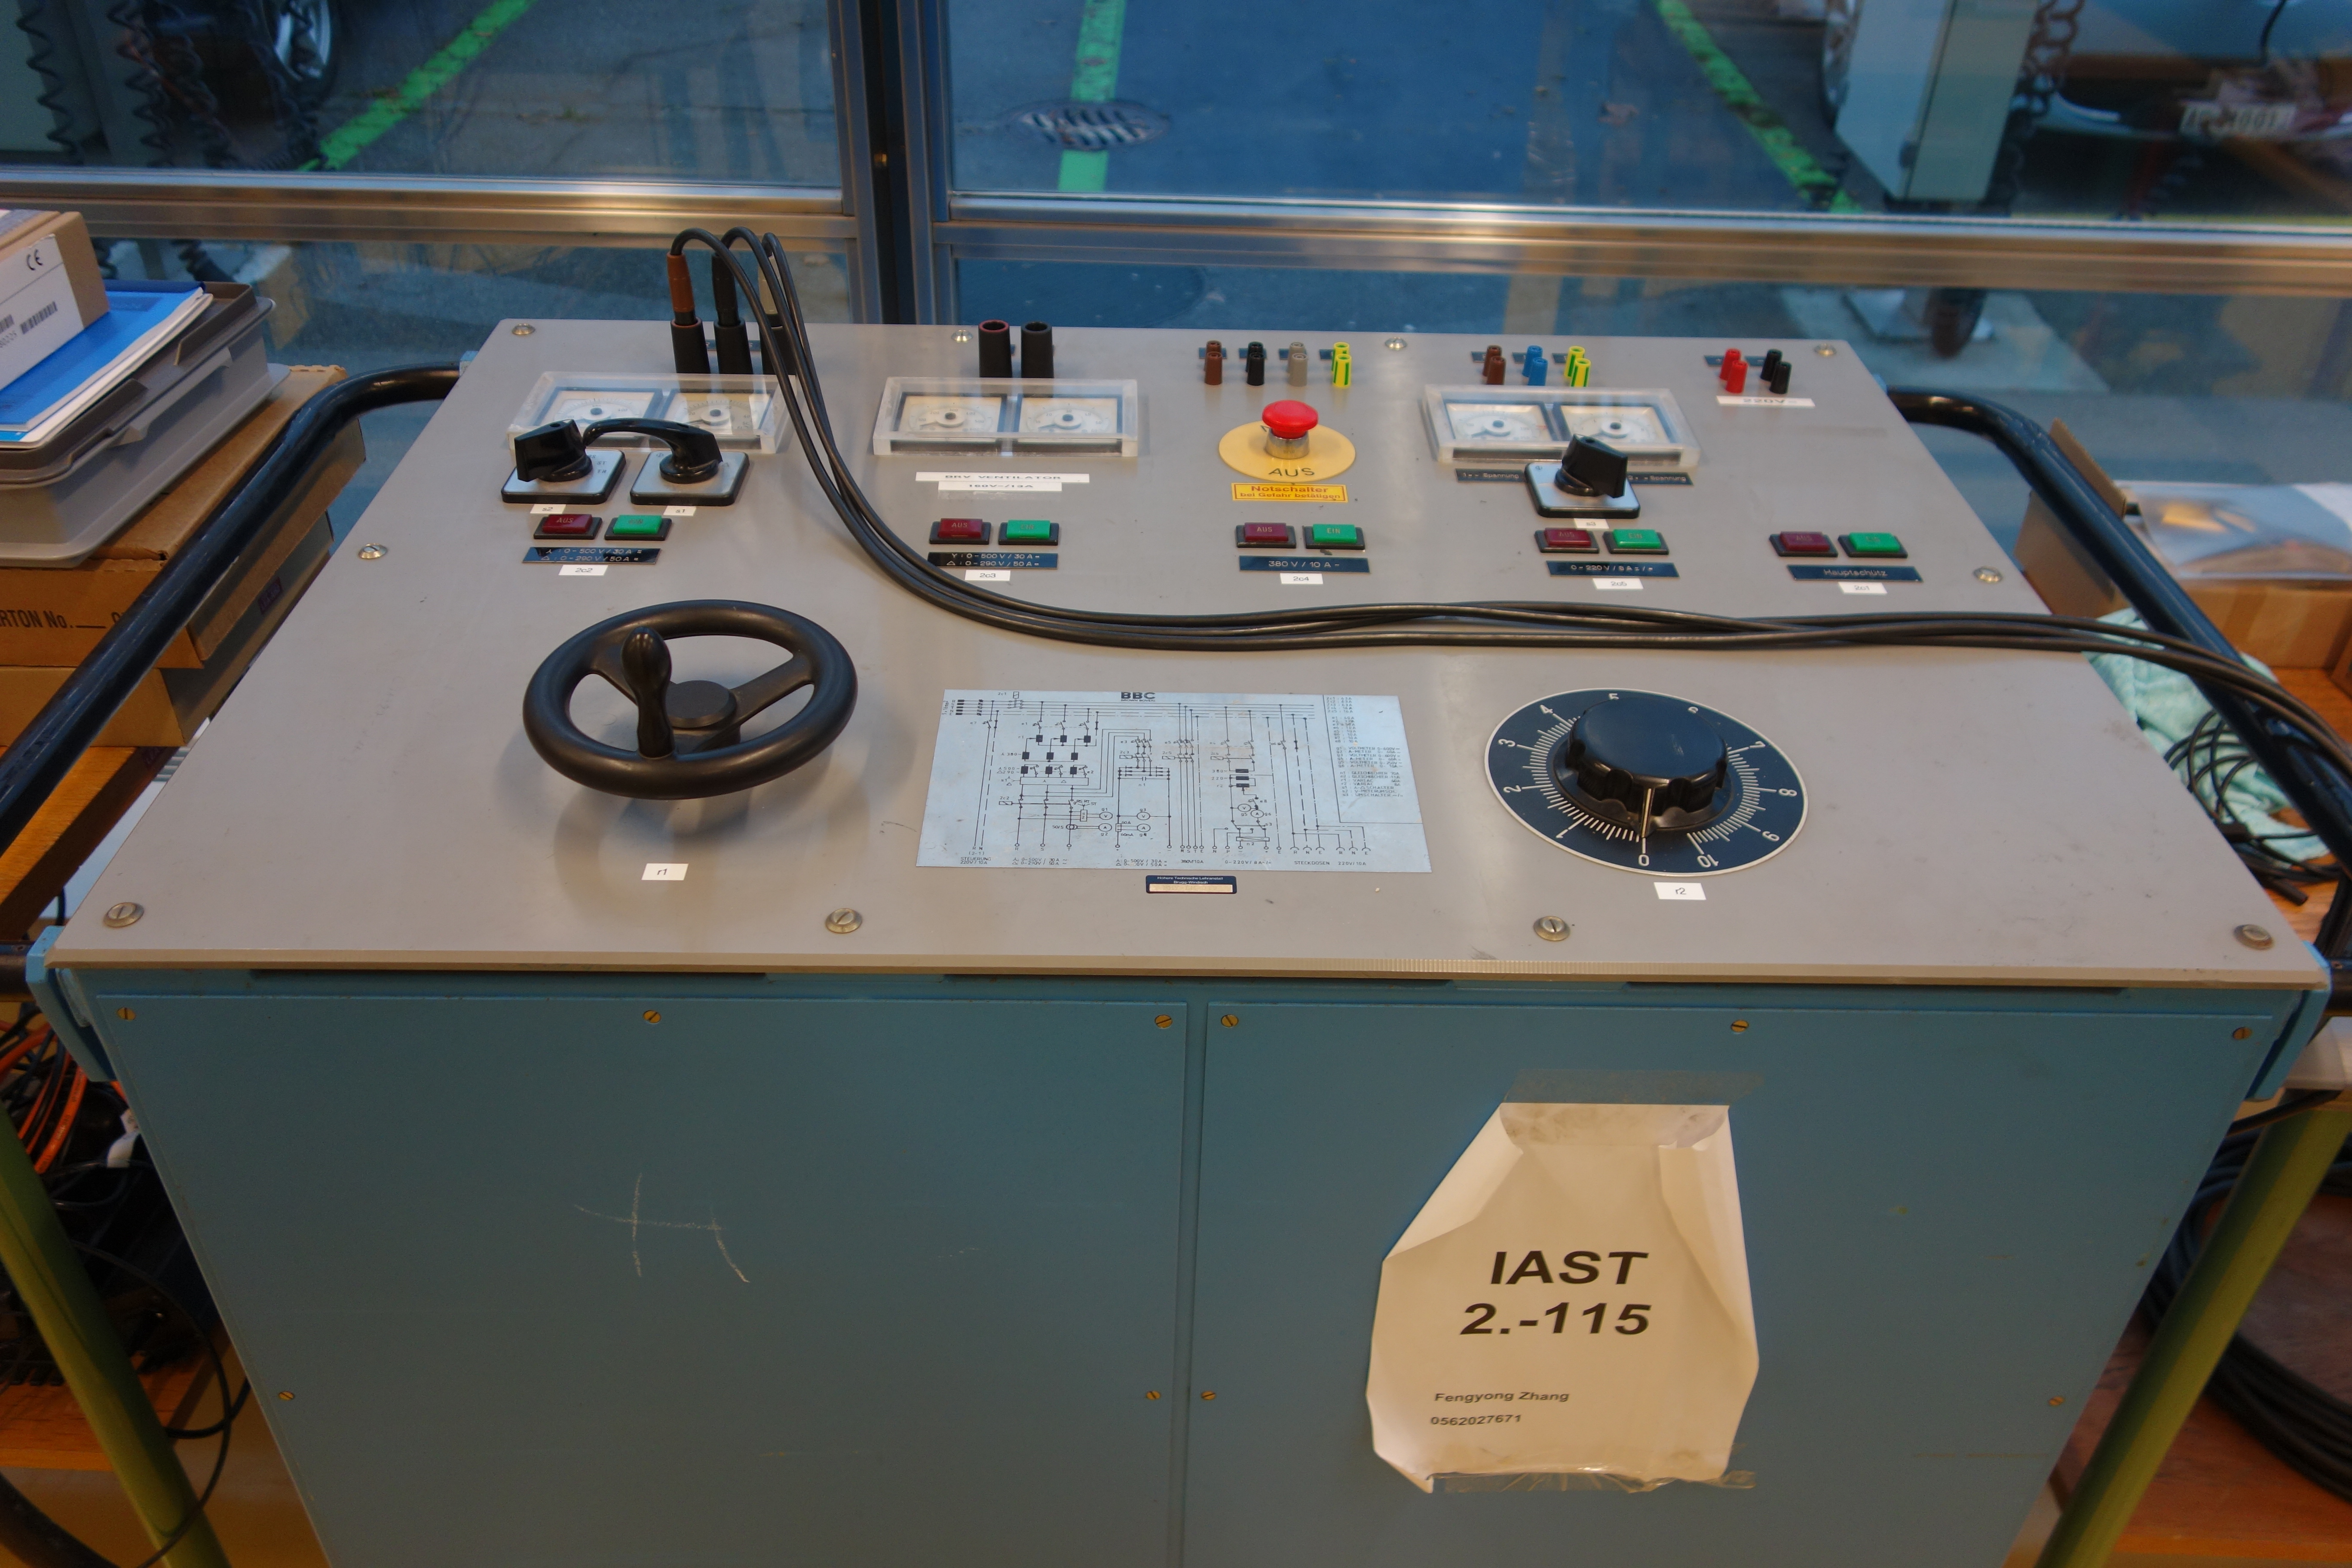
\includegraphics[height=80mm]{Versuchsaufbau/DSC00555.jpg}
		\caption[Variac Versuchsaufbau]{Variac Versuchsaufbau}
		\label{fig:Variac}
	\end{center}
\end{figure}

Die Einspeisung des Variacs erfolgte durch eine CEE-63A Steckdose und ist auf der Abbildung nicht ersichtlich. Die Regulierung des Variacs erfolgt mittels drehen am kleinen schwarzen \glqq Steuerrad\grqq \space (unten links) und gibt bei Dreieckschaltung eine Ausgangsspannung zwischen 0-290V und einen maximalen Strom von 50A. Da unser Motor lediglich eine Betriebsspannung von 96V und im Nennbetrieb einen Strom von deutlich über 100A benötigt, wird ein Transformator nachgeschaltet (Abbildung \ref{fig:Trafo}). Der Anschluss erfolgte Primärseitig und Sekundärseitig in Dreieckschaltung und hat einen sekundären Maximalstrom von $95A_{AC}$ bei $127V_{AC}$. Die Gleichrichtung erfolgt mittels einer B6-Brücke, welche während diesem Projekt selber gebaut wurde. Der Aufbau ist in Abbildung \ref{fig:B6} ersichtlich.

\begin{figure}[H]
	\centering
	\begin{minipage}[H]{.4\linewidth} % [b] => Ausrichtung an \caption
		\centering
		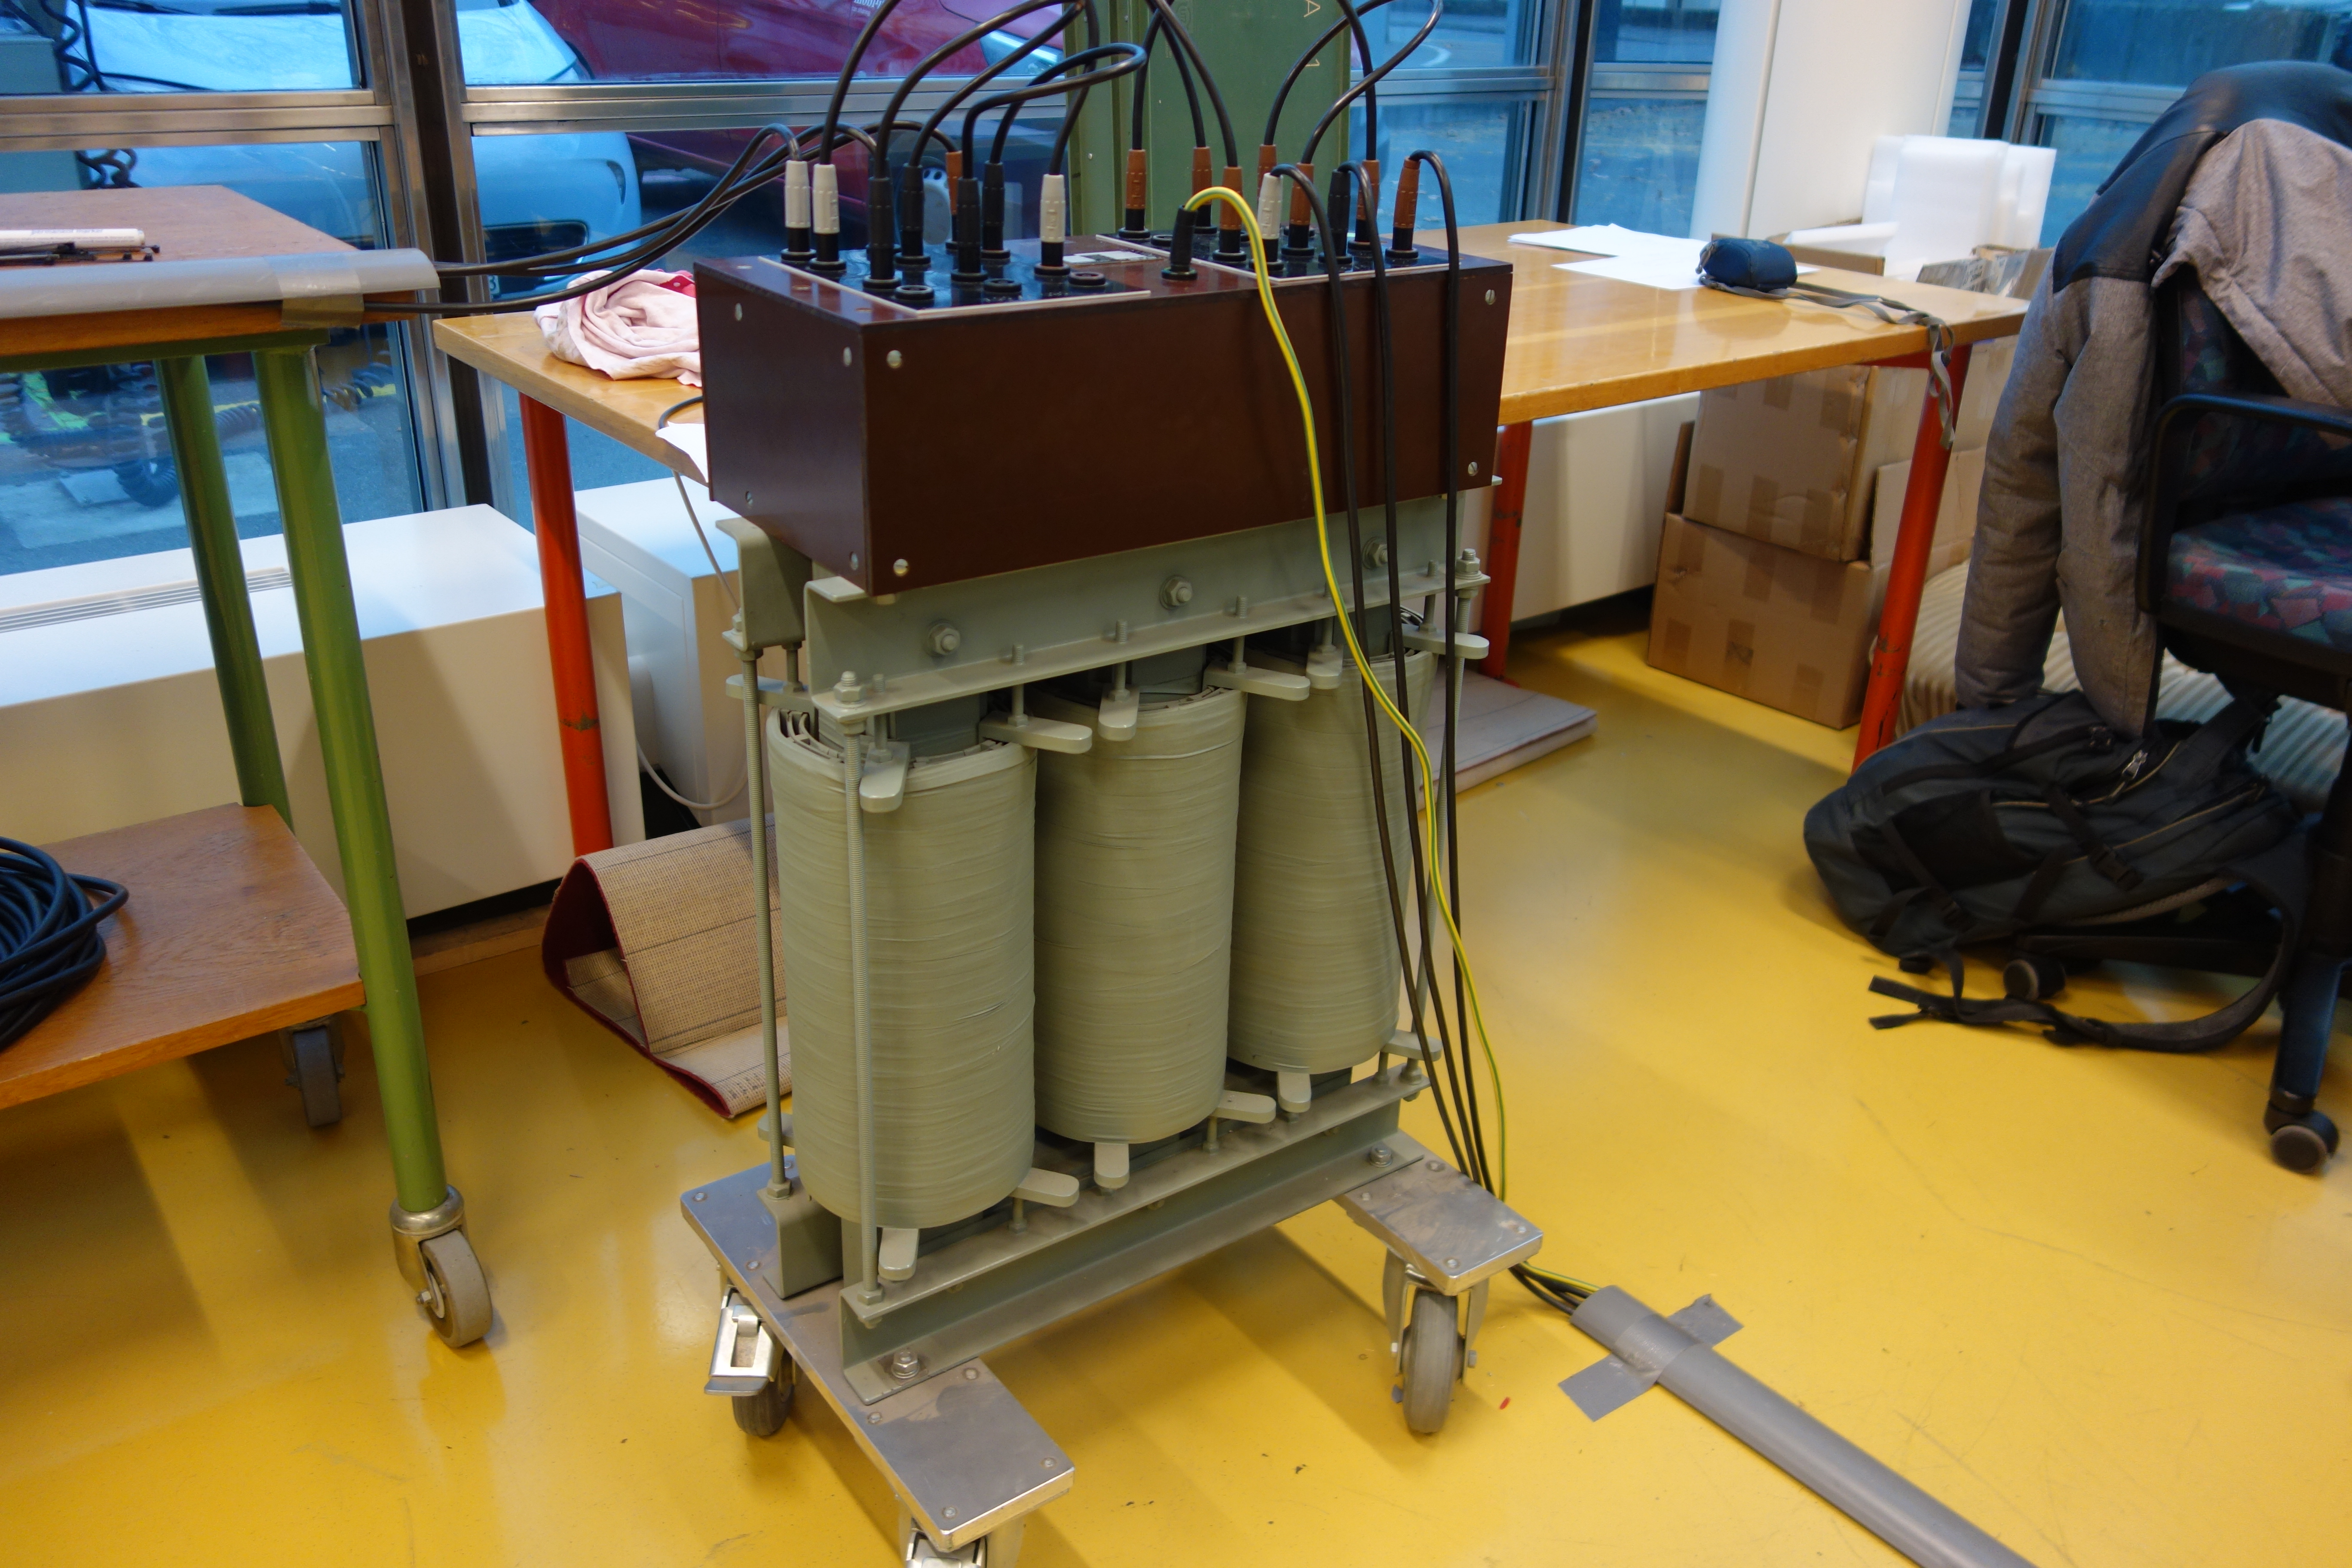
\includegraphics[width=\linewidth]{Versuchsaufbau/DSC00556.jpg}
		\caption[Transformator Versuchsaufbau]{Transformator}
		\label{fig:Trafo}
	\end{minipage}
	\ % Abstand zwischen Bilder
	\begin{minipage}[H]{.4\linewidth} % [b] => Ausrichtung an \caption
		\centering
		\includegraphics[width=\linewidth]{Versuchsaufbau/DSC00547(2).jpg}
		\caption[B6 Gleichrichter]{B6 Gleichrichter}
		\label{fig:B6}
	\end{minipage}
\end{figure}

Die AC-Einspeisung der B6-Brücke erfolgt mittels den drei Klemmen (Braun, Schwarz, Grau) im unteren Bereich. Diese werden auf den eigentlichen Diodengleichrichter (Weiss) und zwei Stützkondensatoren (Blau) geführt.Gemäss der Formel \ref{eq:B6-Id} ergibt sich somit einen maximalen Zwischenkreisstrom auf der DC Seite von $I_{DC}=\frac{95A}{0.8165} =\underline{116.35A}$.
Dieser erhöhte Strom, wird DC-Seitig durch jeweils zwei Hin-, und Rückleiter (Blau und Rot) auf die Motorenansteuerung geführt.\\
Die zwei Elektrolytkondensatoren (Elkos), welche in der Abbildung \ref{fig:Controller} ganz links ersichtlich sind, dienen zur Glättung der Gleichstromversorgung bei hohen Belastungen. Der Controller ist rechts im Bild ersichtlich, dazwischen befindet sich noch ein DC-Relais, welches vom Controller angesteuert wird und die DC-Speissung unterbrechen kann.

\begin{figure}[H]
	\begin{center}
		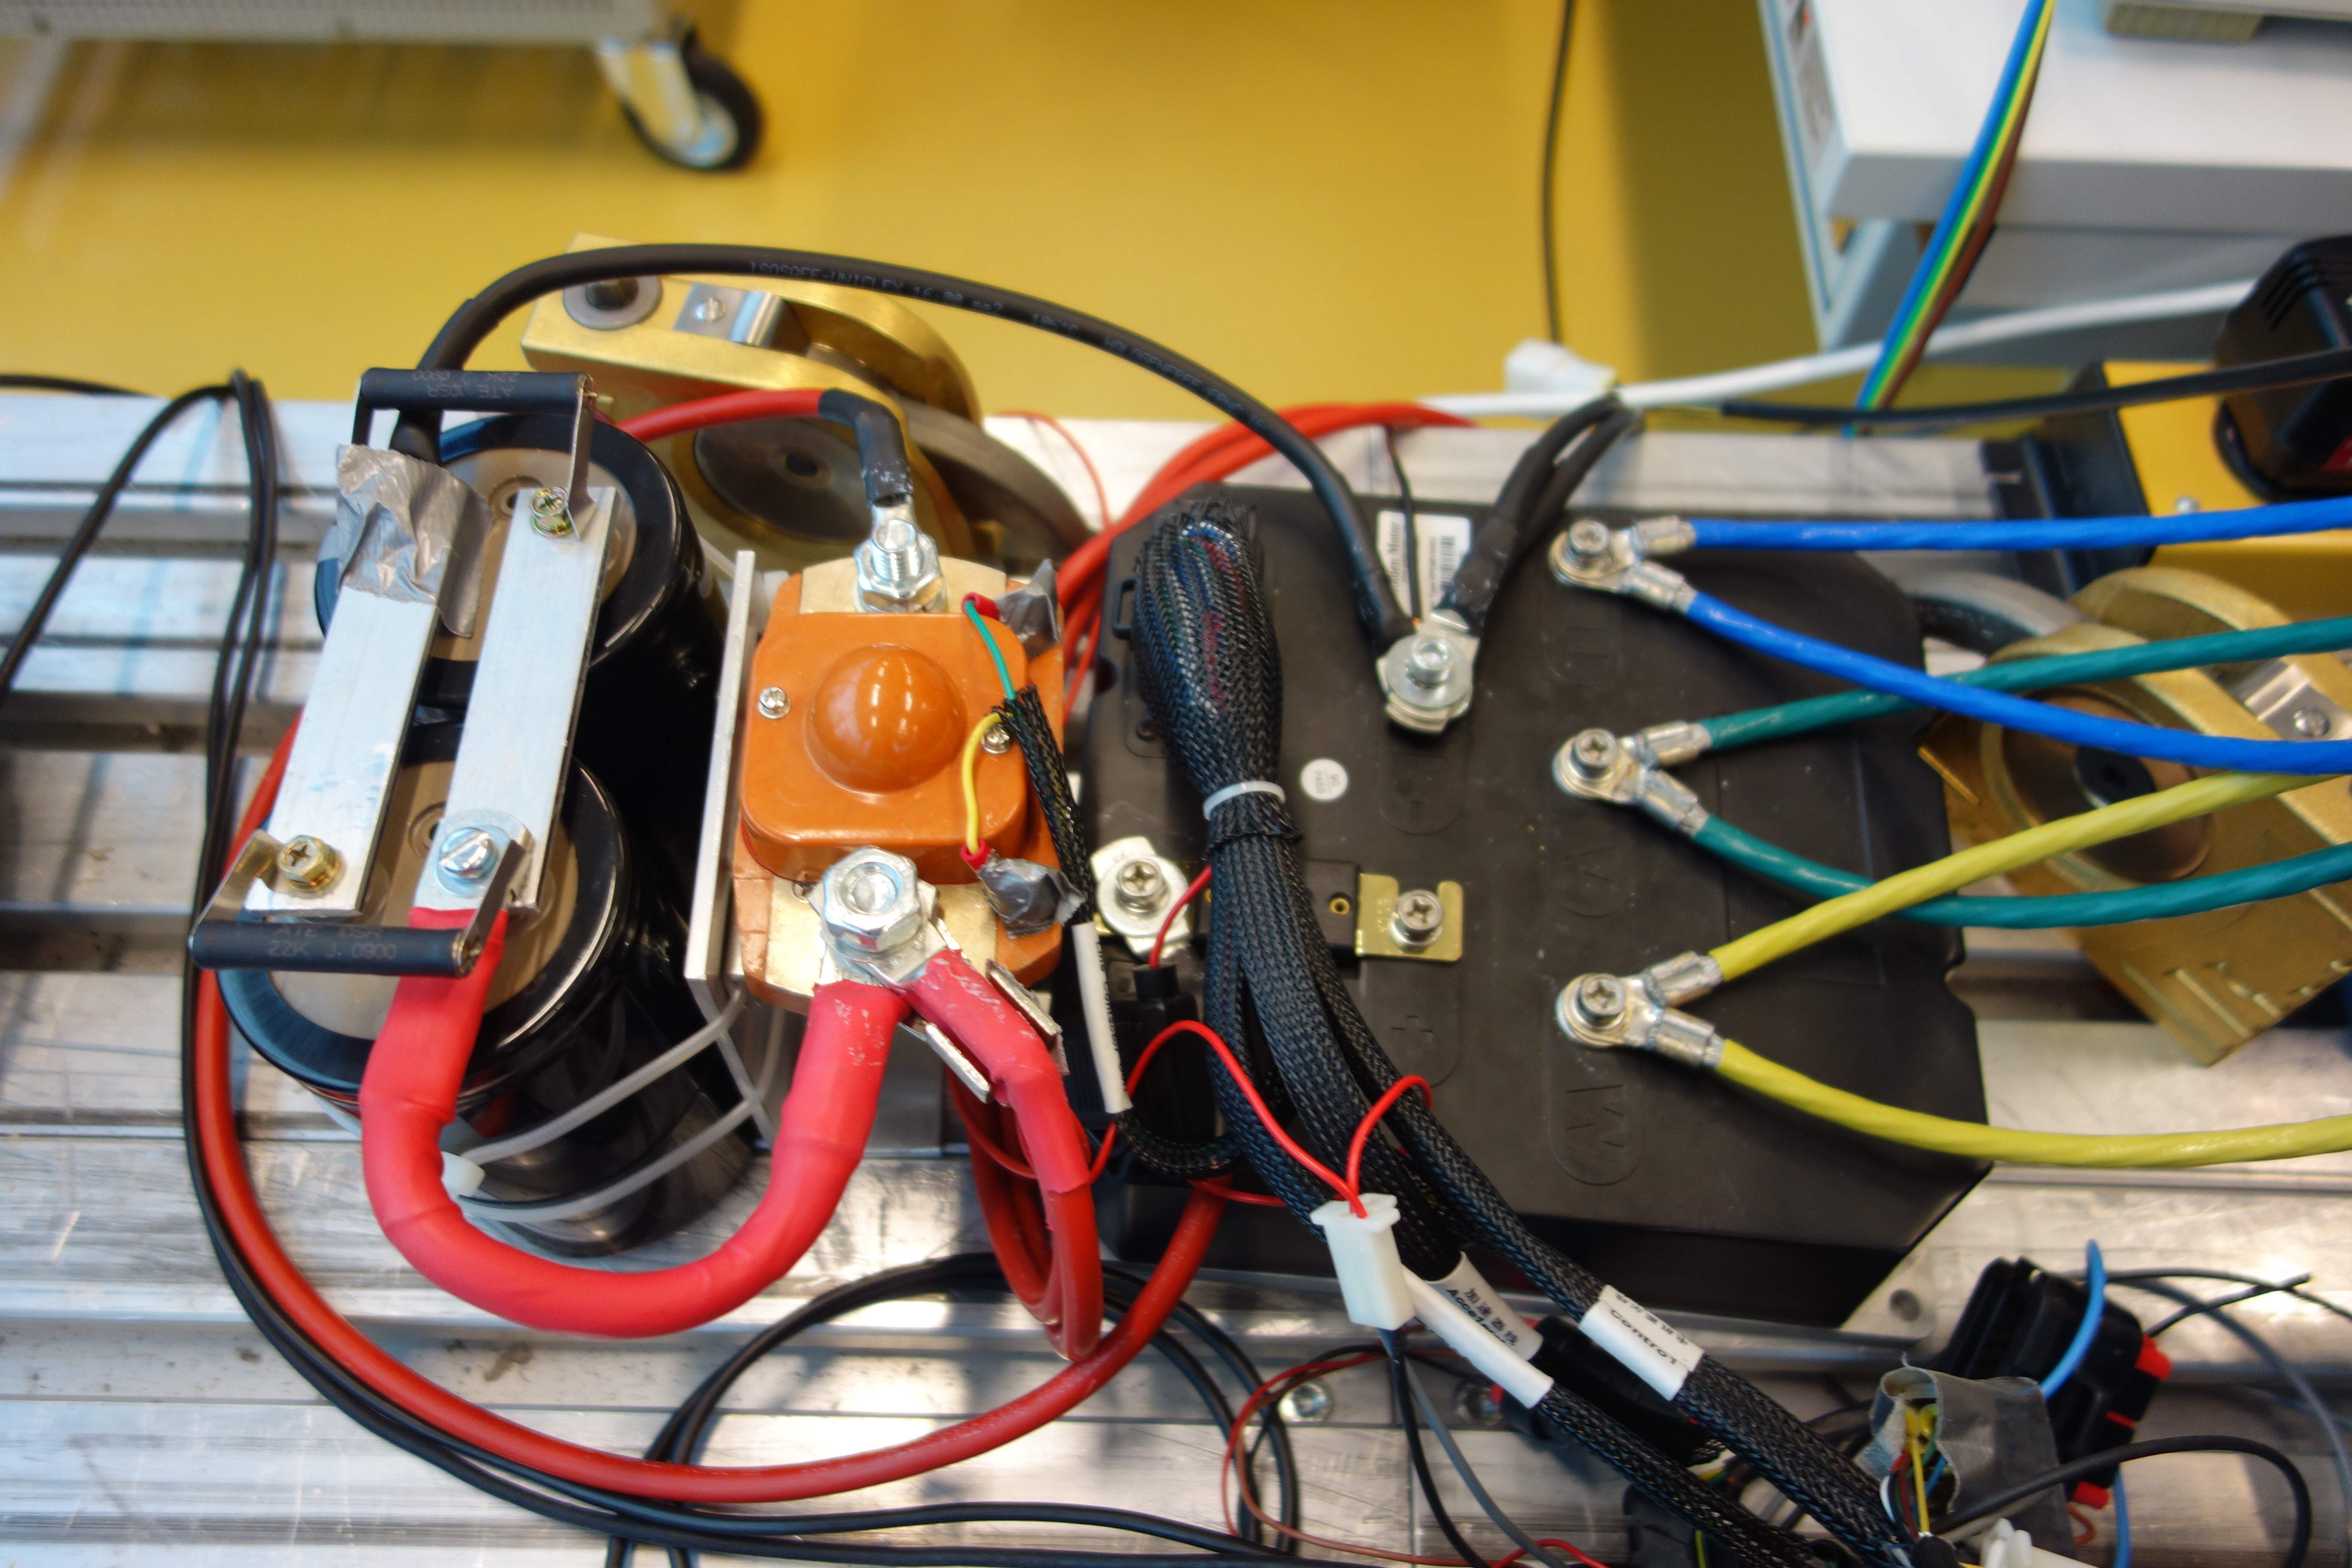
\includegraphics[height=80mm]{Versuchsaufbau/DSC00581.jpg}
		\caption[Controller]{Controller}
		\label{fig:Controller}
	\end{center}
\end{figure}

Tritt ein Fehlerfall auf, kann der Controller mithilfe des DC-Relais die Stromversorgung unterbrechen. Etwas schwer auf der Abbildung zu erkennen sind die Kontakte auf dem Controller. Dieser besitzt eine Sicherung direkt nach der Einspeisung des +Pols. Weiter ist ein geflechteter Kabelbaum ersichtlich (welcher alle Kabel zur Ansteuerung des Controllers beinhaltet) und die farbigen Anschlusskabel des Motors auf der rechten Seite.\\
Aus Sicherheitsgründen wurden alle blanken Elemente mit Klebestreifen isoliert und der Controller, die Elkos und das DC-Relais mit einer Kiste abgedeckt.

Der Drehmoment-Sollwert für die Ansteuerung wurde mit einem Arduino-Controller erzeugt. Dabei wurde der PWM-Ausgang mithilfe eines RC-Tiefpasses in ein Spannungssignal gewandelt. Mithilfe eines Schmitt-Triggers konnte zudem die Drehzahl des Motors gemessen und geregelt werden. Auf der Abbildung \ref{fig:Mikrocontroller} ist das Arduino-Board ersichtlich. Darauf aufgebaut ist eine Experimentierplatine mit drei Taster (rechts) um den Sollwert einzustellen, einem Schmitt-Trigger (mitte) und dem RC-Tiefpass (links).

\begin{figure}[H]
	\begin{center}
		\includegraphics[height=60mm]{Versuchsaufbau/DSC00559.jpg}
		\caption[Controller]{Controller mit Experimentierplatine}
		\label{fig:Mikrocontroller}
	\end{center}
\end{figure}

Wie anfänglich bereits beschrieben wurde, wurde der verwendete BLDC Motor mit einer ASM gekoppelt. Die Anordnung ist in Abbildung \ref{fig:MotorenLueftung} links dargestellt. Damit diese zwei Maschinen überhaupt miteinander gekoppelt werden konnten, musste einerseits die Welle des BLDC Motors (links) auf das Niveau der ASM (rechts) angehoben werden und andererseits mussten einige Anpassungen an der Kupplung getätigt werden. Da der DC-Motor über eine Welle mit Zollmass verfügt, musste die Öffnung einer Kupplung ausgebohrt werden. Weiter verfügt die ASM über keine Nut, weshalb die andere Seite der Kupplung zur Befestigung mit einem Gewinde versehen werden musste. Die Befestigung erfolgt mittels zwei M8-Schraube, welche auf die Welle drücken. Für den Berührungsschutz sorgt eine Plexiglasscheibe über der mechanischen Verbindung.


\begin{figure}[H]
	\begin{center}
		\includegraphics[width=\linewidth]{Versuchsaufbau/MotorLueft.png}
		\caption[Motoren Aufbau und Motorenlüftung]{Motoren Aufbau (links) und Motorenlüftung (rechts)}
		\label{fig:MotorenLueftung}
	\end{center}
\end{figure}

Leider weisst der verwendete Motor eine schlechte Eigenkühlung auf, wodurch zusätzliche Ventilatoren notwendig sind. In unseren Temperaturtests \ref{subsec:Temperatur} wurden zur Kühlung externe 110mm Ventilatoren verwendet. In Abbildung \ref{fig:MotorenLueftung} Grafik rechts, wurde die Anordnung seitlich und hinter dem Motor gewählt.


Damit überhaupt Leistungsversuche möglich sind, muss neben dem Gleichstrommotor auch die ASM angesteuert werden. Hierbei diente ein Frequenzumrichter (Abbildung \ref{fig:Frequenzumformer}) mit integrierter Netzschaltung. Die Versorgung erfolgt mittels einem CEE-32A Stecker und ist dementsprechend mit 32A abgesichert.

\begin{figure}[H]
	\centering
	\begin{minipage}[h]{.4\linewidth} % [b] => Ausrichtung an \caption
		\centering
		\includegraphics[height=100mm]{Versuchsaufbau/DSC00575.jpg}
		\caption[Frequenzumformer]{Frequenzumformer}
		\label{fig:Frequenzumformer}
	\end{minipage}
	\quad % Abstand zwischen Bilder
	\begin{minipage}[h]{.4\linewidth} % [b] => Ausrichtung an \caption
		\centering
		\includegraphics[width=\linewidth]{Versuchsaufbau/SteuerungRegelung.png}
		\caption[Ansteuerung und Regelung]{Ansteuerung und Regelung}
		\label{fig:AnsteuerungRegelung}
	\end{minipage}
\end{figure}

 Die Ansteuerung ist in Abbildung \ref{fig:AnsteuerungRegelung} ersichtlich, wobei die obere Grafik die Steuerungseinheit abbildet. In dieser können verschiedene Ansteuerungsverfahren (Frequenz oder Moment gesteuert) eingestellt werden. Ausserdem können diverse Parameter in der dazugehörigen Code-Tabelle verändert werden, wodurch die ASM optimal angesteuert werden kann. Durch die Veränderung der maximalen Frequenz kann indirekt die Maximaldrehzahl bestimmt werden. Die Frequenz wird durch eine Widerstandsänderung durch ein externes Potentiometer gegeben (Abbildung \ref{fig:AnsteuerungRegelung} unten rechts). Die externe Eingabe kann zudem die Steuerung aktivieren und die Drehrichtung ändern (unten links).
